\chapter{Model Accuracy Results}
\label{ch:AccuracyResult}
In this chapter, all test result would be represented and discussed here. Most of those test results try to predict one year stock price. The addition result can be found in Appendix~


\section{Using 4 years historical data}

The test slot is from 2010-01-06 to 2015-01-06, the first four year data (from 2010-01-06 to 2014-01-05) are training dataset (986 transaction days), the remaining used to act as testing data (test size is 248).\\


The average stock price over this period is showed in table~\ref{tb:avg20142015} and the RMSE comparison is in figure~\ref{fg:4yearpredict1}, \ref{fg:4yearpredict2} and \ref{fg:4yearpredict3}. Average CDC info can be found in table~\ref{tb:averageCDC1}.\\


\begin{table}[h]
	\centering
	\begin{tabular}{|l|l|l|l|}
		\hline
		\textbf{Stock Symbol} & \textbf{Average Price(HKD)} & \textbf{Stock Symbol} & \textbf{Average Price (HKD)} \\ \hline
		\textbf{0001.HK}      & 94.9379262096775       & \textbf{0006.HK}      & 68.62278225806452      \\ \hline
		\textbf{0002.HK}      & 63.25927419354843      & \textbf{0007.HK}      & 1.316129032258065      \\ \hline
		\textbf{0003.HK}      & 19.05447125000001      & \textbf{0008.HK}      & 4.466854838709676      \\ \hline
		\textbf{0004.HK}      & 55.95322580645161      & \textbf{0009.HK}      & 0.6356521739130431     \\ \hline
		\textbf{0005.HK}      & 80.08870967741933      & \textbf{0010.HK}      & 39.71733870967743      \\ \hline
	\end{tabular}
	\caption{Average Stock Price (from 2014-01-06 to 2015-01-06)}
	\label{tb:avg20142015}
\end{table}

%\begin{figure}[h]
%	\centering
%	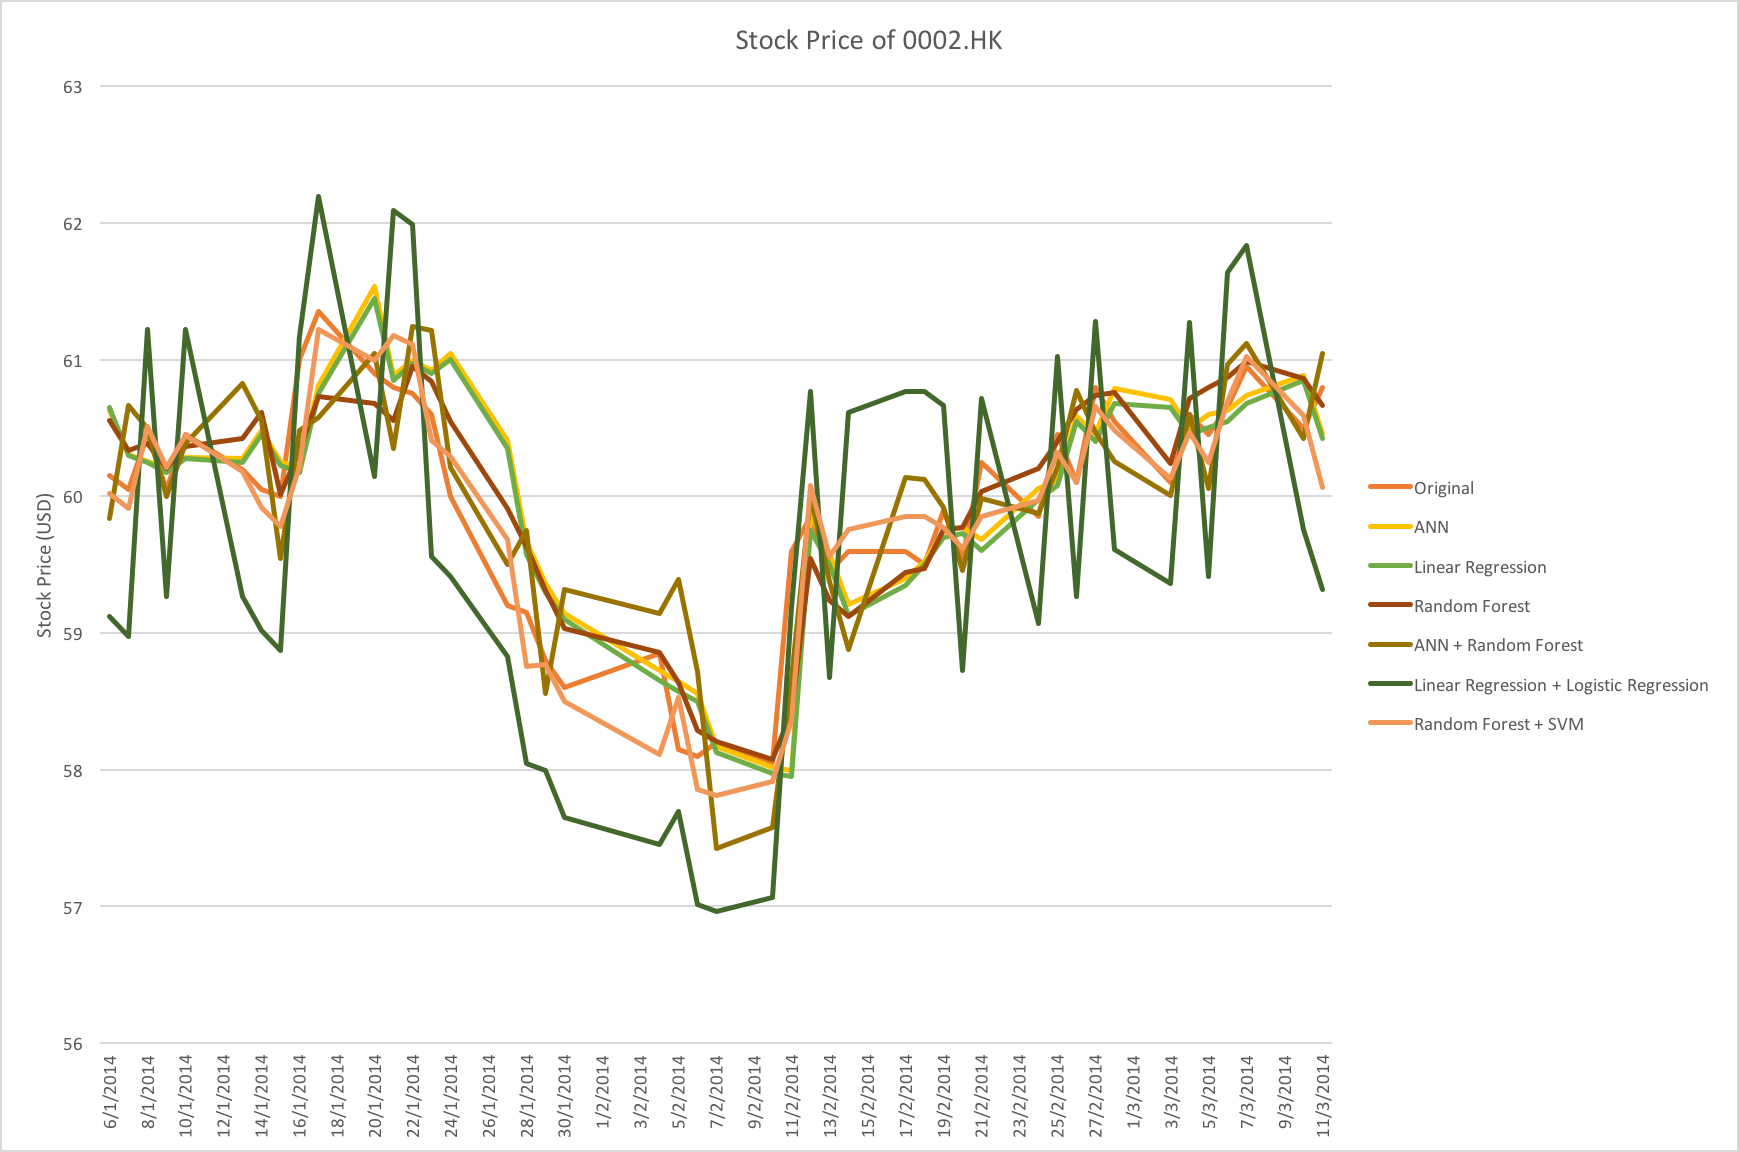
\includegraphics[width=.8\textwidth]{Result/20102015/0002}
%	\caption{Sample Predict prices of 0002.HK}
%\end{figure}

\begin{figure}[h]
	\centering
	\includegraphics[width=.8\textwidth]{Result/20102015/ME}
	\caption{Testing result in time period 2014-01-07 to 2015-01-06}
	\label{fg:4yearpredict1}
\end{figure}

\begin{figure}[h]
	\centering
	\subfigure[RMSE]{
		\centering
		\includegraphics[width=.8\textwidth]{Result/20102015/RMSE}
	}
	\subfigure[CDC]{
		\centering
		\includegraphics[width=.8\linewidth]{Result/20102015/CDC}
	}
	\caption{Testing result in time period 2014-01-07 to 2015-01-06 (continue)}
	\label{fg:4yearpredict2}
\end{figure}

\begin{figure}[h]
	\centering
	\subfigure[MAPE]{
		\centering
		\includegraphics[width=.8\textwidth]{Result/20102015/MAPE}
	}
	\subfigure[HMSE]{
		\centering
		\includegraphics[width=.8\linewidth]{Result/20102015/HMSE}
	}
	\caption{Testing result in time period 2014-01-07 to 2015-01-06 (continue)}
	\label{fg:4yearpredict3}
\end{figure}

\begin{table}[h]
	\centering
	\begin{tabular}{|l|l|}
		\hline
		\textbf{Algorithm} & \textbf{Average CDC} \\ \hline
		\textbf{ANN} & 46.52\% \\ \hline
		\textbf{Linear Regression} & 46.61\% \\ \hline
		\textbf{Random Forest} & 63.20\% \\ \hline
		\textbf{\begin{tabular}[c]{@{}l@{}}Linear Regression \\ + Logistic Regression\end{tabular}} & 60.14\% \\ \hline
		\textbf{Random Forest + SVM} & 60.14\% \\ \hline
		\textbf{ANN + Random Forest} & 65.82\% \\ \hline
	\end{tabular}
	\caption{Average CDC in time period 2010-01-06 to 2015-01-06}
	\label{tb:averageCDC1}
\end{table}
\clearpage

The best learning algorithm under this circumstance is Random Forest, which has the second best CDC (In figure~\ref{fg:4yearpredict2}.b and table~\ref{tb:averageCDC1} the best algorithm is a combined method whose trend model is also based on Random Forest) and lowest error in amount prediction. And as both linear classifiers, the CDC result of Logistic Regression and SVM are almost same\\


For combination method, random forest algorithm is also the best model to predict stock price change amount. The performance of classifiers is also acceptable.


\section{Using 3 years historical data}

This time slot is from 2010-01-06 to 2014-01-06, the first three year data (from 2010-01-06 to 2013-01-06) are training dataset (train size is 743), the remaining used to act as testing data (test size is 244).\\


The average stock price over this period is showed in table~\ref{tb:avg20132014} and the RMSE comparison is in figure~\ref{fg:3yearpredict1}, \ref{fg:3yearpredict2} and \ref{fg:3yearpredict3}. Average CDC info can be found in table~\ref{tb:averageCDC2}.\\
\begin{table}[h]
	\centering
	\begin{tabular}{|l|l|l|l|}
		\hline
		\textbf{Stock Symbol} & \textbf{Average Price(HKD)} & \textbf{Stock Symbol} & \textbf{Average Price (HKD)} \\ \hline
		\textbf{0001.HK}      & 83.44622379       & \textbf{0006.HK}      & 68.2534274193548      \\ \hline
		\textbf{0002.HK}      & 64.5012096774194     & \textbf{0007.HK}      & 1.31673267326733      \\ \hline
		\textbf{0003.HK}      & 22.1624665322581      & \textbf{0008.HK}      & 3.55899193548387      \\ \hline
		\textbf{0004.HK}      & 66.6220647773279      & \textbf{0009.HK}      & 0.752991071428572     \\ \hline
		\textbf{0005.HK}      & 84.7485887096774      & \textbf{0010.HK}      & 42.6689516129032      \\ \hline
	\end{tabular}
	\caption{Average Stock Price (from 2013-01-06 to 2014-01-06)}
	\label{tb:avg20132014}
\end{table}

\begin{figure}[h]
	\centering
	\includegraphics[width=.8\textwidth]{Result/3120102014/ME}
	\caption{Testing result in time period 2013-01-07 to 2014-01-06}
	\label{fg:3yearpredict1}
\end{figure}

\begin{figure}[h]
	\centering
	\subfigure[RMSE]{
		\centering
		\includegraphics[width=.8\textwidth]{Result/3120102014/RMSE}
	}
	\subfigure[CDC]{
		\centering
		\includegraphics[width=.8\linewidth]{Result/3120102014/CDC}
	}
	\caption{Testing result in time period 2013-01-07 to 2014-01-06 (continue)}
	\label{fg:3yearpredict2}
\end{figure}

\begin{figure}[h]
	\centering
	\subfigure[MAPE]{
		\centering
		\includegraphics[width=.8\textwidth]{Result/3120102014/MAPE}
	}
	\subfigure[HMSE]{
		\centering
		\includegraphics[width=.8\linewidth]{Result/3120102014/HMSE}
	}
	\caption{Testing result in time period 2013-01-07 to 2014-01-06 (continue)}
	\label{fg:3yearpredict3}
\end{figure}

\begin{table}[h]
	\centering
	\begin{tabular}{|l|l|}
		\hline
		\textbf{Algorithm} & \textbf{Average CDC} \\ \hline
		\textbf{ANN} & 46.33\% \\ \hline
		\textbf{Linear Regression} & 46.50\% \\ \hline
		\textbf{Random Forest} & 59.12\% \\ \hline
		\textbf{\begin{tabular}[c]{@{}l@{}}Linear Regression \\ + Logistic Regression\end{tabular}} & 63.55\% \\ \hline
		\textbf{Random Forest + SVM} & 63.54\% \\ \hline
		\textbf{ANN + Random Forest} & 65.82\% \\ \hline
	\end{tabular}
	\caption{Average CDC in time period 2013-01-07 to 2014-01-06}
	\label{tb:averageCDC2}
\end{table}
\clearpage

Composed learning model performed better in CDC test (in table~\ref{tb:averageCDC2}). Two linear classifiers share similar performance in this test. ANN and Linear Regression are also not trustworthy method to predict stock change direction\\


Random Forest alone and Linear + Logsitic Regression model turns out to be an unreliable choice to predict stock price in this test for some stock (like 0009.HK and 0007.HK). However, almost every method reach its worst performance when handle this two stocks, which on the other way shows that those model are not suitable for stock with average price less than.\\


The overall performance of using 3 years as historical data is better than that of 4 years, which means that 3 years may be more suitable as training period.